\documentclass[10pt,a4paper]{article}
\usepackage[utf8]{inputenc}
\usepackage[spanish]{babel}
\usepackage{amsmath}
\usepackage{amsfonts}
\usepackage{amssymb}
\usepackage{makeidx}
\usepackage{graphicx}
\usepackage[hidelinks]{hyperref}
\usepackage[left=2cm,right=2cm,top=2cm,bottom=2cm]{geometry}
\author{Luis Osvaldo Cervantes Martinez\\Miguel Angel Xamie Diaz Fuentes\\Raul Jimenez Cortes\\Ulises Isaac Reyes Alvarez\\4.B Ing. Mecatrónica\\Mtro. Carlos Enrique Morán Garabito\\"Sistemas Electrónicos de Interfaz"}
\title{Diagrama eléctrico de la interfaz de potencia}

\begin{document}
\maketitle
\begin{figure}[hbtp]
\centering

\includegraphics[scale=2]{Pictures/UPZMG.png}
\end{figure}

\newpage
\section{Introducción}
\textbf{Objetivos}
\begin{itemize}
\item Desarrollar un pwm (pulse-width modulation)
\item Observar el funcionamiento del pwm
\item Hacer funcionar el puente de diodos con el pwm
\end{itemize}

\textbf{Marco teórico}\\
PWM \\
Hablamos de la función PWM como abreviatura de la modulación por ancho de pulsos, algo que se ha convertido en una práctica habitual de los interruptores de potencia modernos, controlando la energía de inercia. Esta acción tiene en cuenta la modificación del proceso de trabajo de una señal de tipo periódico. Puede tener varios objetivos, como tener el control de la energía que se proporciona a una carga o llevar a cabo la transmisión de datos.\\

La función PWM requiere de un circuito en el cual hay distintas partes bien diferenciadas entre sí. El comparador es lo que se convierte en el nexo, contando con una salida y un total de dos entradas distintas. A la hora de configurarlo tenemos que tener en cuenta que una de las dos entradas se centra en dar espacio a la señal del modulador. Por su lado, la segunda entrada tiene que estar vinculada con un oscilador de tipo de dientes de sierra para que la función se pueda llevar a cabo con éxito. La señal que proporciona el oscilador con dientes es lo que determina la salida de la frecuencia. Es un sistema que ha dado buenas demostraciones de funcionar, convirtiéndose en un recurso muy utilizado en cuanto a la disponibilidad de recursos energéticos.\\

Tenemos que tener en cuenta distintos factores a la hora de hablar de los usos prácticos de la función PWM. Con el paso de los años y desde que la PWM entrara en vigor, las placas madre contaron con sensores de temperatura, consultables desde la bios del equipo. A partir de ese momento se impuso reducir el ruido de la CPU, haciendo que el ordenador reaccionara de distintas maneras en base al contexto. Si por ejemplo, estamos utilizando el equipo con el objetivo de descargar archivos, como demos de videojuegos, realmente el ordenador no necesita una potencia superior a la mínima. En estos casos la CPU no se calienta, no necesita el ventilador y se debe evitar gastar energía de forma innecesaria.\\

Cuando montamos un ordenador que deba poder ofrecer un rendimiento de primer nivel, pensamos en incluir la mayor potencia de ventilación, para que en situaciones críticas estos ventiladores puedan funcionar a toda máquina con el objetivo de evitar problemas en el equipo. Pero esta configuración se desaprovecha en momentos como en el ejemplo citado de la descarga de archivos. En estas situaciones no es necesario que el ventilador gire a toda velocidad, sino que se puede mantener en los niveles mínimos. La función PWM es una manera de regularlo. Para perfeccionar esto se le añadió un cable adicional que manda una señal de la velocidad a la que está funcionando el ventilador. La placa base se encarga de regular la velocidad a la que debe ir el ventilador en cada momento. Si el equipo se calienta mucho, le dice con una señal que debe trabajar más. Para ello hay que configurar el ordenador desde la bios siempre pensando en obtener los menores índices de ruido.\\ 

\begin{figure}[hbtp]
\centering
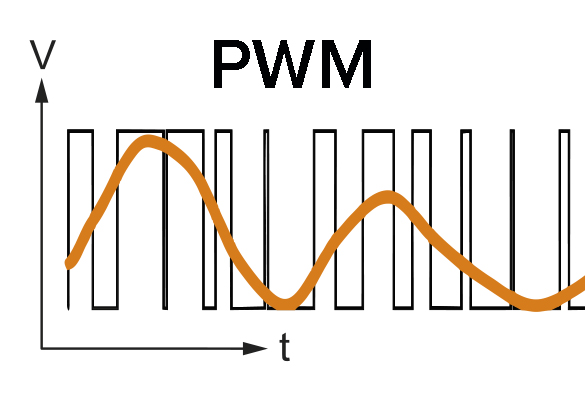
\includegraphics[scale=0.3]{Pictures/pwm.jpg}
\caption{PWM}
\end{figure}

\footnote{Universidad Politécnica de la Zona Metropolitana de Guadalajara}


\newpage
\section{Materiales y equipo}

\begin{itemize}
\item Protoboard
\item Cables para protoboard
\item Caimanes
\item Transistor NPN TIP41C / TIP31
\item Fuente de alimentación 1.5V, 9V  y 12V
\item Resitencias 47K$\Omega$, 1k$\Omega$ y 100$\Omega$
\item Capacitores 10$\mu$F, 100$\mu$F y 220$\mu$F
\item Bobinas 2.5mH hechas a mano o bobinas de transformador
\item LED's 
\item MOSFET TIP112
\item Potenciómetros 10k$\Omega$ y 5k$\Omega$
\item Amplificador operacional LM555
\end{itemize}
\footnote{Universidad Politécnica de la Zona Metropolitana de Guadalajara}

\newpage
\section{Desarrollo}
\textbf{1. Primero vamos a desarrollar un pwm}
Déspues de haber investigado en paginas web encontramos un circuito el cual nos basaremos para realizar nuestra práctica: 
\begin{figure}[hbtp]
\centering
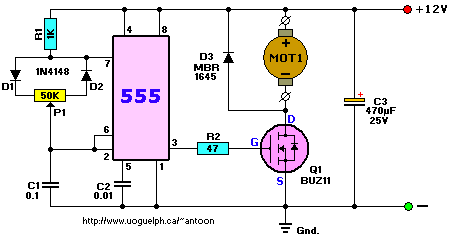
\includegraphics[scale=1]{Pictures/555.PNG}
\caption{Circuito pwm}
\end{figure}

Una vez teniendo armado el circuito en la protoboard, verificando que todo este bien, como se muestra a continuación: 
\begin{figure}[hbtp]
\centering
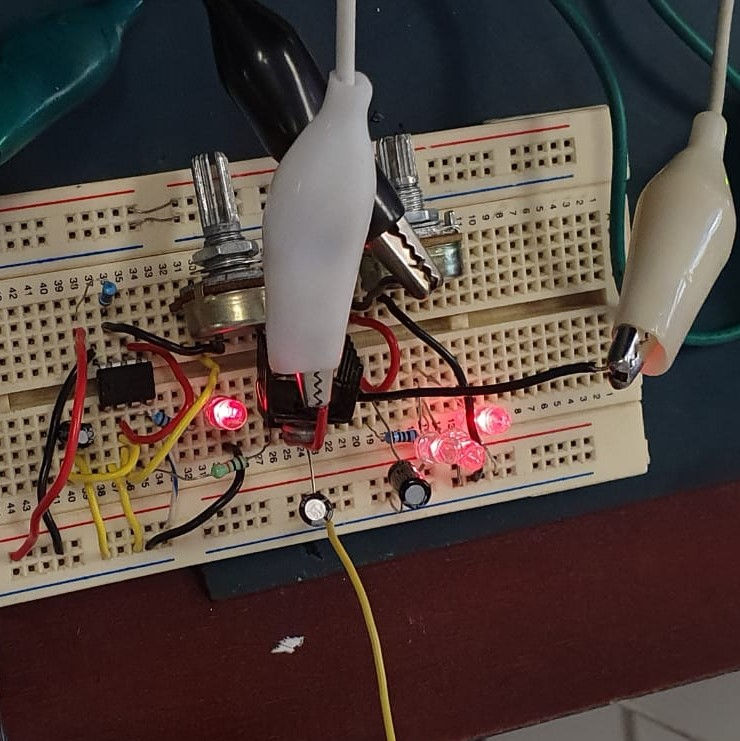
\includegraphics[scale=0.5]{Pictures/pwm.jpeg}
\caption{Circuito armado en protoboard}
\end{figure}

Vamos a realizar la segunda parte del circuito que es el puente de diodos: 

\footnote{Universidad Politécnica de la Zona Metropolitana de Guadalajara}

\newpage
\begin{figure}[hbtp]
\centering
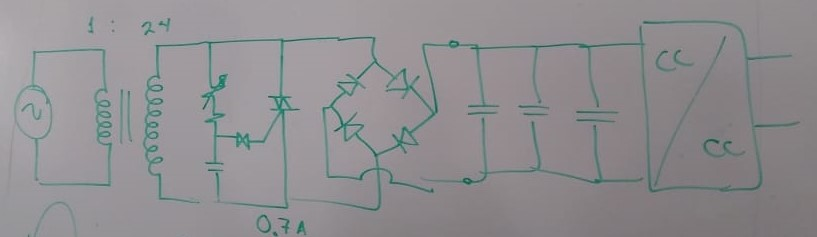
\includegraphics[scale=0.7]{Pictures/Puente.jpeg}
\caption{Circuito Puente de diodos}
\end{figure}

Quedandonos de la siguiente manera: 
\begin{figure}[hbtp]
\centering
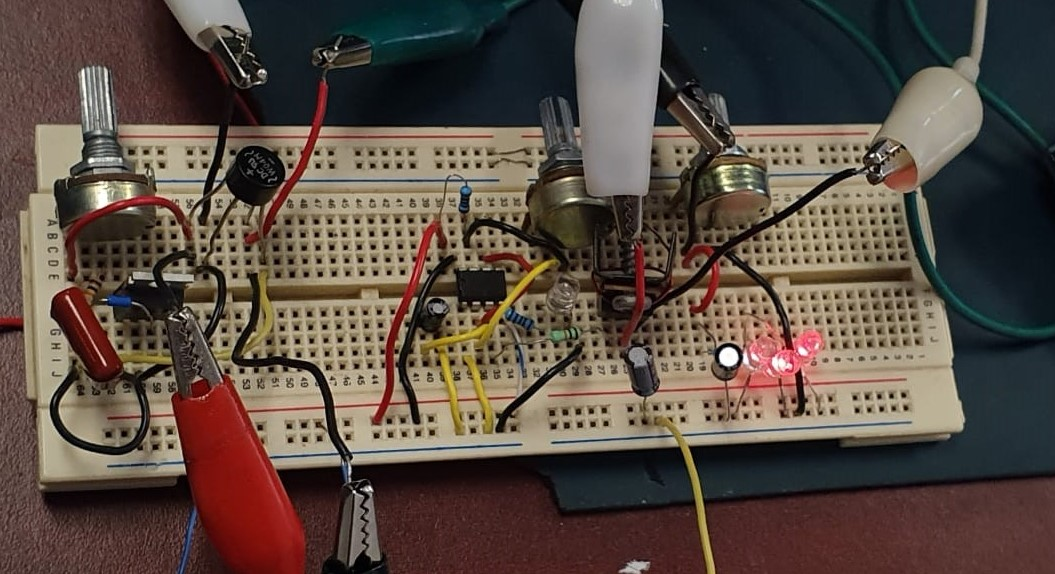
\includegraphics[scale=0.3]{Pictures/Pwm3.jpeg}
\caption{Circuito armado}
\end{figure}

Quedandonos listo para conectar nuestras fuentes y poder observar el funcionamiento que es simplemente un reductor de voltaje, para encender los 3 LED's de la siguiente práctica: 
\begin{figure}[hbtp]
\centering
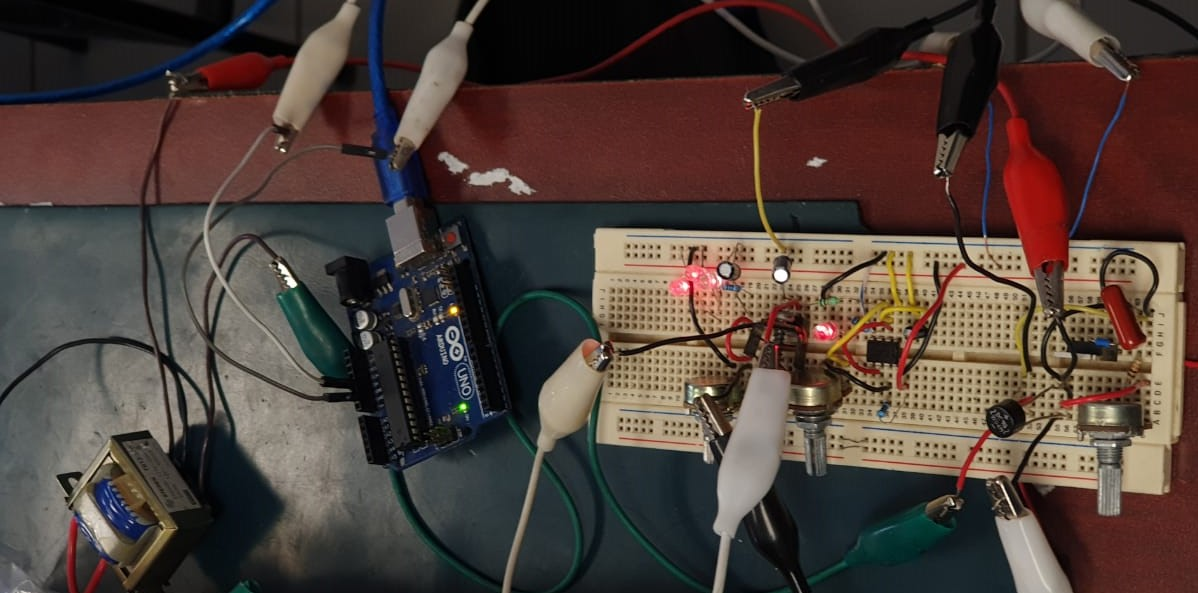
\includegraphics[scale=0.3]{Pictures/pwm1.jpeg}
\caption{Circuito pwm con puente de diodos}
\end{figure}

\footnote{Universidad Politécnica de la Zona Metropolitana de Guadalajara}

\newpage
\section{Conclusiones}
\textbf{Luis Osvaldo Cervantes Martinez}\\
El puente de diodos o también llamado puente rectificador o puente de Graetz es un circuito rectificador de onda completa, el cual fue el objeto principal de esta práctica en la cual el puente de diodos requiere de cuatro diodos rectificadores o diodos de potencia conectados en serie en forma de puente, la principal ventaja de este circuito de puente rectificador permite la rectificación de onda completa de un transformador por lo que es una práctica muy importante y de mucha utilidad para futuros proyectos.\\

\textbf{Raul Jimenez Cortés}\\
Mi conclusión de esta práctica es que pudimos entender de manera en cómo actuaban los leds a través del potenciómetro de una manera distinta a la practica 9 ya que esta conjunta con ella, en esta los leds no parpadean al momento de aumentar la intensidad como lo solían hacer en la nueva ya que en esta se le hizo un puente de diodos  haciendo un modelo boost con el cual pudimos dar a concluir esta práctica con el objetivo que se esperaba a cabo.\\

\textbf{Ulises Isaac Reyes Alvarez}\\
En está práctica aprendimos a desarrollar un pwm(modulación por ancho de pulsos) para poder desarrollar nuestra práctica mediante un puente de diodos, tras la activación de un TRIAC y un DIAC para el encendido de LED's, y el funcionamiento adecuado del puente de diodos. Teniendo un circuito boost, generando mayor voltaje de salida, haciendo que los LED's enciendan aún mas o menos. 

\footnote{Universidad Politécnica de la Zona Metropolitana de Guadalajara}

\newpage
\begin{figure}[hbtp]
\centering
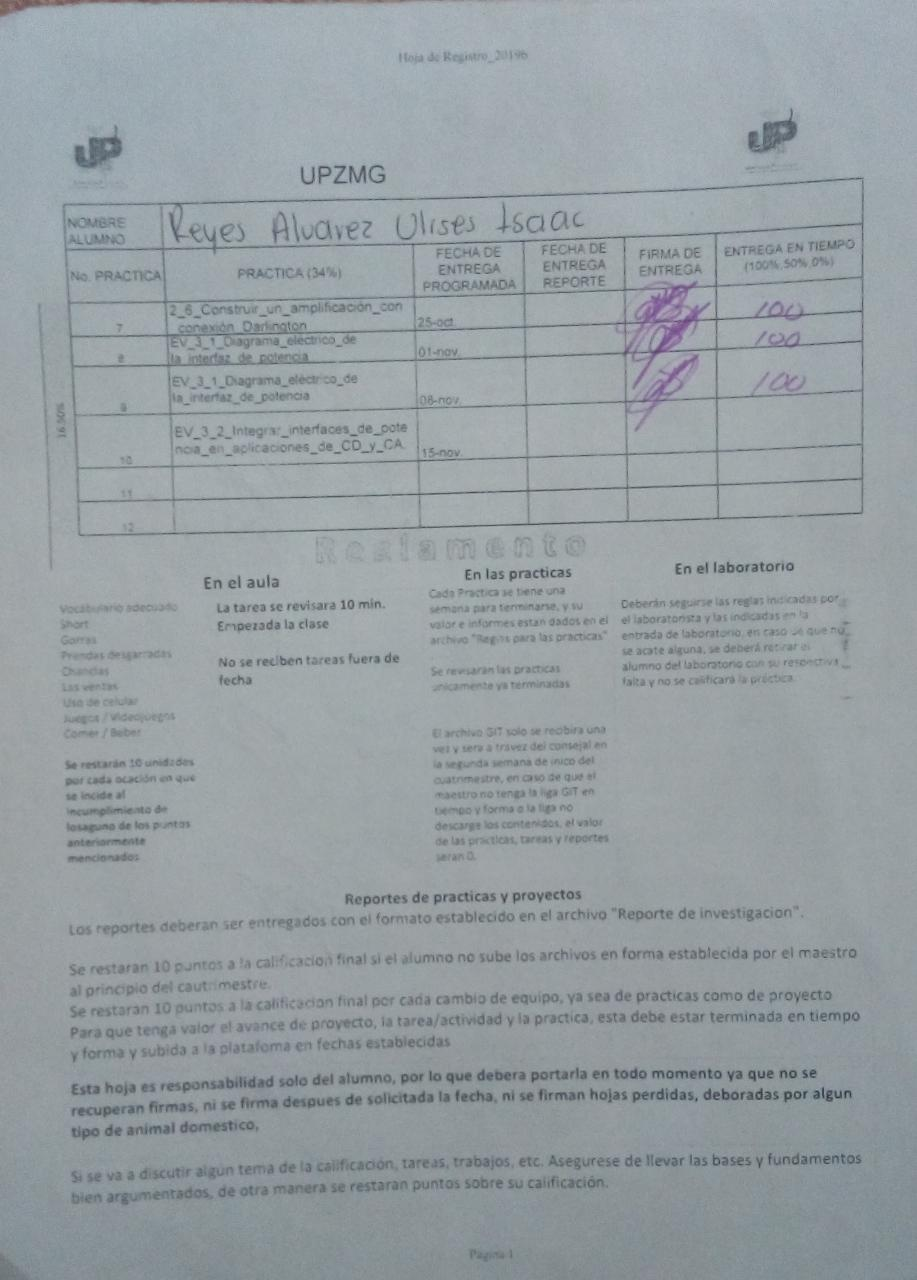
\includegraphics[scale=0.4]{Pictures/ULISES.png}
\caption{Ulises Isaac Reyes Alvarez}
\end{figure}
\footnote{Universidad Politécnica de la Zona MEtropolitana de Guadalajara}

\end{document}